% Copyright (C) Data Structures and Algorithms Team.
\chapter{Introduction}

\section{What this book is, and what it isn't}
This book provides implementations of common and uncommon algorithms in pseudo code which is language independent and provides for easy porting to most imperative programming languages, it is not a definitive book on the theory of data structures and algorithms.

For the most part this book presents implementations devised by the authors themselves based on the concepts by which the respective algorithms are based upon so it is more than possible that our implementations differ from those considered the norm.

You should use this book alongside a book on the same subject, but one that contains formal proofs of the algorithms in question. In this book we use the abstract big oh notation to depict the run time complexity of algorithms so that the book appeals to a larger audience.

\section{Assumed knowledge}
We have written this book with few assumptions of the reader, however we have, nonetheless had to make some assumptions to keep the book as concise and approachable as possible. The assumptions are that the reader is familiar with the following:

\begin{enumerate}
\item Big Oh notation
\item An imperative programming language
\item Familiarity with object oriented concepts
\end{enumerate}

\subsection{Big Oh notation}
For run time complexity analysis we use big Oh notation extensively so it is vital that you are familiar with the general concepts to determine which is the best algorithm for you in certain scenarios. We have chosen to use big Oh notation for a few reasons, however the most important is that it provides an abstract measurement in which we can judge the performance of algorithms without using mathematical proofs.

Figure \ref{algorithmic_runtime_expansion} shows some of the run times to depict how important choosing an efficient algorithm is, for the sanity of our graph we have omitted cubic $O(n^{3})$, and exponential $O(2^{n})$ run times. Cubic, and exponential algorithms should only ever be used for very small problems (if ever!), avoid them if feasibly possible. 

\begin{figure}
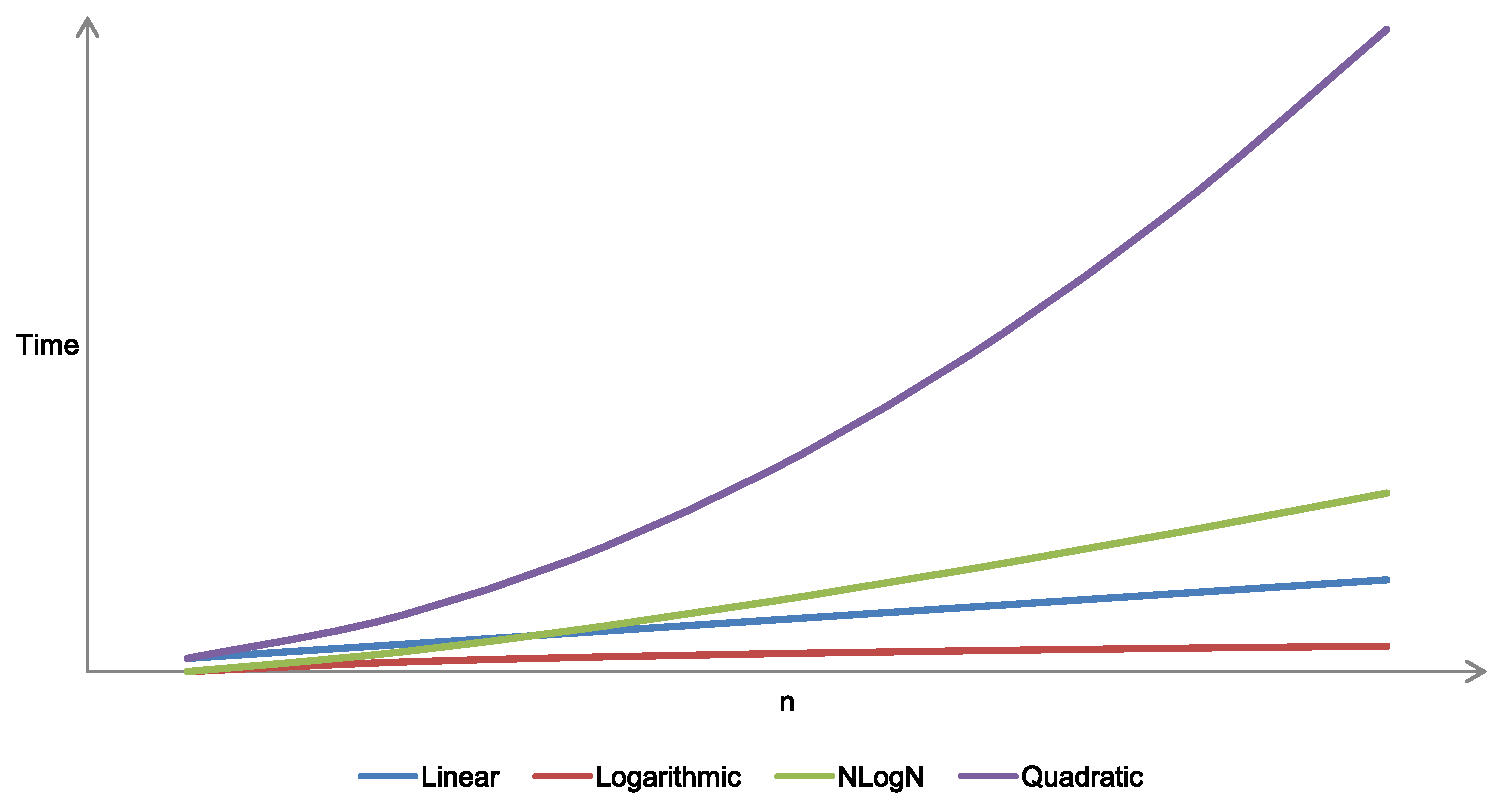
\includegraphics[scale=0.5]{intro_runtimes}
\caption{Algorithmic run time expansion} \label{algorithmic_runtime_expansion}
\end{figure}

The following list explains some of the most common big Oh notations:

\begin{enumerate}
\item[$O(1)$]: constant, the operation requires no major computation, e.g. adding a node to the end of a linked list when we maintain a tail pointer.
\item[$O(n)$]: linear, the run time complexity is proportionate to the size of $n$.
\item[$O(log~n)$]: logarithmic, normally associated with algorithms that break the problem into smaller chunks per each invocation, e.g. searching a binary search tree.
\item[$O(n~log~n)$]: just $n~log~n$, usually associated with an algorithm that breaks the problem into smaller chunks per each invocation, and then takes the results of these smaller chunks and stitches them back together, e.g. quick sort.
\item[$O(n^{2})$]: quadratic, e.g. bubble sort.
\item[$O(n^{3})$]: cubic, very rare.
\item[$O(2^{n})$]: exponential, incredibly rare.
\end{enumerate}

\subsection{Imperative programming language}
All examples are given in a pseudo imperative coding format and so the reader must know the basics of some imperative mainstream programming language to port the examples effectively, we have written this book with the following target languages in mind:

\begin{enumerate}
\item C++
\item C\#
\item Java
\end{enumerate}

The reason that we are explicit in that we require all readers to be familiar with an imperative language is simple - all our implementations are based on imperative style thinking, if you are a functional programmer you will need to apply various aspects from the functional paradigm to produce solutions with respect to your functional language whether it be Haskell, F\#, OCaml, etc.


Two of the languages that we have listed (C\#, and Java) target virtual machines which provide various things like security sand boxing, and memory management via garbage collection algorithms - to port our implementations to these languages is trivial. When porting to C++ you must remember to use pointers for certain things, e.g. a linked list node has a reference to the next node, this is an example where we are describing the solution in the context of a managed environment so in C++ you will want to interpret the reference as a pointer to the next node and so on. For programmers who have a fair amount of experience with their respective language these subtleties will present no issue which is why we really do emphasise that the reader must be comfortable with at least one imperative language to have a greater amount of success when porting the pseudo implementations in this book.


It is essential that the user is familiar with primitive imperative language constructs before reading this book otherwise you will just get lost, some algorithms presented in this book can be confusing to follow even for experienced programmers!

\subsection{Object oriented concepts}
For the most part in this book we do not use features that are specific to any one language, and we never provide data structures or algorithms that work on generic types, this is to make the samples as easy to follow as possible, however in order to appreciate the designs of our data structures you will need to be familiar with the following object oriented (OO) concepts:

\begin{enumerate}
\item Inheritance
\item Encapsulation
\item Polymorphism
\end{enumerate}

This is required even more so if you are planning on looking at the C\# target that we have implemented (more on that in \S\ref{intro_source_code}) which makes extensive use of the above listed OO concepts. As a final note it is also desirable that the reader is familiar with interfaces as the C\# target uses interfaces throughout the sorting algorithms.

\section{Pseudo code}
Throughout this book we use pseudo code do describe our solutions, for the most part interpreting the pseudo code is trivial as it looks very much like a more abstract C++, or C\#, however there are a few things to point out:

\begin{enumerate}
\item Pre-conditions should be enforced always; and
\item Post-conditions represent the result of applying algorithm $a$ to data structure $d$; and
\item The type of parameters is inferred; and
\item All primitive language constructs are explicitly begun and ended
\end{enumerate}

If an algorithm has a return type it will be presented in the post-condition, however in many cases the return type is obvious and as a result this information may be omitted from the post-condition for brevity.

Most algorithms in this book require parameters, and because we assign no explicit type to those parameters the type is inferred from the contexts in which it is used, and the operations performed upon it. The biggest clue however of what type the parameter is can be attained simply from its name, e.g. $n$ is a pseudo name for number and so you can assume unless otherwise stated that $n$ translates to an integer that has the same number of bits as a WORD on a $32$ bit machine, similarly $l$ is a pseudo name for a list where a list is a resizeable array (e.g. a vector).

The last major point of reference is that we always explicitly end a language construct, e.g. if we wish to close the scope of a \textit{for} loop then we will explicitly state \textit{end for} rather than leaving the interpretation of when scopes are closed to the reader which may in some complex cases lead to ambiguity.

\begin{tabbing}
1)  \textbf{alg}\= \textbf{orithm} AlgorithmName($n$) \\
2)  \> \textbf{Pre:}~~$n$ is the value to compute the factorial of \\
3)  \> ~~~~~~~~$n \geq 0$ \\
4)  \> \textbf{Post:}~the factorial of $n$ has been computed \\
5)  \> // ... \\
n) \textbf{end} AlgorithmName \\
\end{tabbing}

The example above describes an algorithm by the name of \textit{AlgorithmName}, and takes a single parameter $n$ which is a number. What follows the algorithm signature are any pre and post conditions, you should always enforce the pre-conditions of an algorithm when porting them to your language of choice.

Because everything we describe is not language dependant you will need to make your own mind up on how to best handle pre-conditions. Just so that you know though in the C\# target we have implemented we consider non-conference to pre-conditions exceptional cases, particularly because we can throw some information back to the caller and tell them why the algorithm has failed to be invoked. 

\section{Tips for working through the examples}
As with most books you get out what you put in and so we recommend that in order to get the most out of this book you work through each algorithm with a pen and paper to track things like variable names, recursive calls etc.

The best way to work through algorithms is to setup a table, and in that table give each variable its own column and continuously update the value of the variables, this will help you keep track of, and visualise the mutations that are occurring throughout the algorithm. Often while working through algorithms in such a way you can intuitively map relationships between data structures very easily rather than trying to work out a few values on paper and the rest in your head. We suggest you put everything on paper irrespective of how trivial some variables and calculations may be so that you always have a point of reference.

When dealing with recursive algorithm traces we recommend you do the same as the above, but also have a table that records function calls and who they return to. This approach is a far cleaner way than drawing out an elaborate map of function calls with arrows to one another, which, from experience gets large quickly and simply makes things more complex to follow. Track everything in a simple, and systematic way to make your time studying the implementations far easier.

\section{Book outline}
We have split this book into two parts:

\begin{enumerate}
\item[Part 1:] Provides discussion and pseudo implementations of common and uncommon data structures; and
\item[Part 2:] Provides algorithms of varying purpose's from sorting algorithms to algorithms that operate on strings.
\end{enumerate}

The reader doesn't have to read the book sequentially from beginning to end, chapters can be read independently from one another. For chapters in part 1 we advise that the reader reads each chapter in it's entirety, however in part 2 you can get away by just reading the section of a chapter that describes the algorithm you are interested in.

For all readers we recommend that before looking at any algorithm you quickly look at Appendix \ref{symbol_defs} which contains a table listing the various symbols used within our algorithms and their meaning.

\section{Where can I get the code?} \label{intro_source_code}
This book doesn't provide any code specifically aligned with it, however we do actively maintain an open source project\footnote{All readers are encouraged to provide suggestions, feature requests, and bugs etc so we can further improve our implementations.} that houses a C\# implementation of all the pseudo code listed. The project is named \textit{Data Structures and Algorithms} (DSA) and can be found at the following url: \url{http://codeplex.com/dsa}.

\section{Final messages}
We have only a few final messages to the reader that we hope you digest before you embark on reading this book, they are:

\begin{enumerate}
\item Understand how the algorithm works first in an abstract sense; and
\item Always work through the algorithms on paper to understand how they achieve their outcome
\end{enumerate}

If you always follow the above key points then you will get the most out of this book.
